\chapter{Overview}
\label{cp:overview}
\section{Data Collection Methodology}
The data collection for this study occurred between October 2021 and mid-January 2024, with one author conducting observations from October 2021 to mid-January 2024 and the other author from September 2022 to mid-January 2024. The process included random observations carried out consistently during these periods, and certain bird species were identified based on their distinctive calls. In January 2024, special observations were conducted, encompassing the entire university to ensure comprehensive documentation of all bird species.
\\
To create the final comprehensive checklist of bird species, the data collected by both authors was merged.

\begin{importantbox}
\subsection{Limitations}
 Random observations inherently possess limitations, compounded by the potential for overlooking certain university regions due to challenging accessibility. However the special observations conducted at end should have minimized the effects of this to some extent. Furthermore, observations across various areas may lack uniform frequency, introducing variability. Additionally, two authors conducted overlapping yet distinct observations during disparate time periods.
\end{importantbox}

\section{Climate}
University is located in the Low country Wet Zone. The area experiences an annual precipitation, primarily brought by the southwest monsoon from May to September. Additionally, inter-monsoon rains occur in March-April and October-November. Although January tends to be drier, there is no distinctly defined dry season. The average temperature hovers around 27 degrees Celsius, accompanied by a relative humidity of approximately 90\%.

\section{Eco-systems}
The observation reveals that various bird species exhibit a diverse range of habitat preferences, encompassing both entirely natural ecosystems and human-made ecosystems situated within and in close proximity to the university.

The neighboring regions of Bolgoda Lake and the Kaju Kele area can be categorized as natural ecosystems, whereas spaces like gardens and the university playground fall under the classification of human-made ecosystems. Notably, even in entirely artificial environments, the study records the presence of certain bird species while some of the species are strictly restricted to certain areas of the university.

\begin{figure}[!htpb]
    \centering
    \begin{subfigure}{0.45\textwidth}
        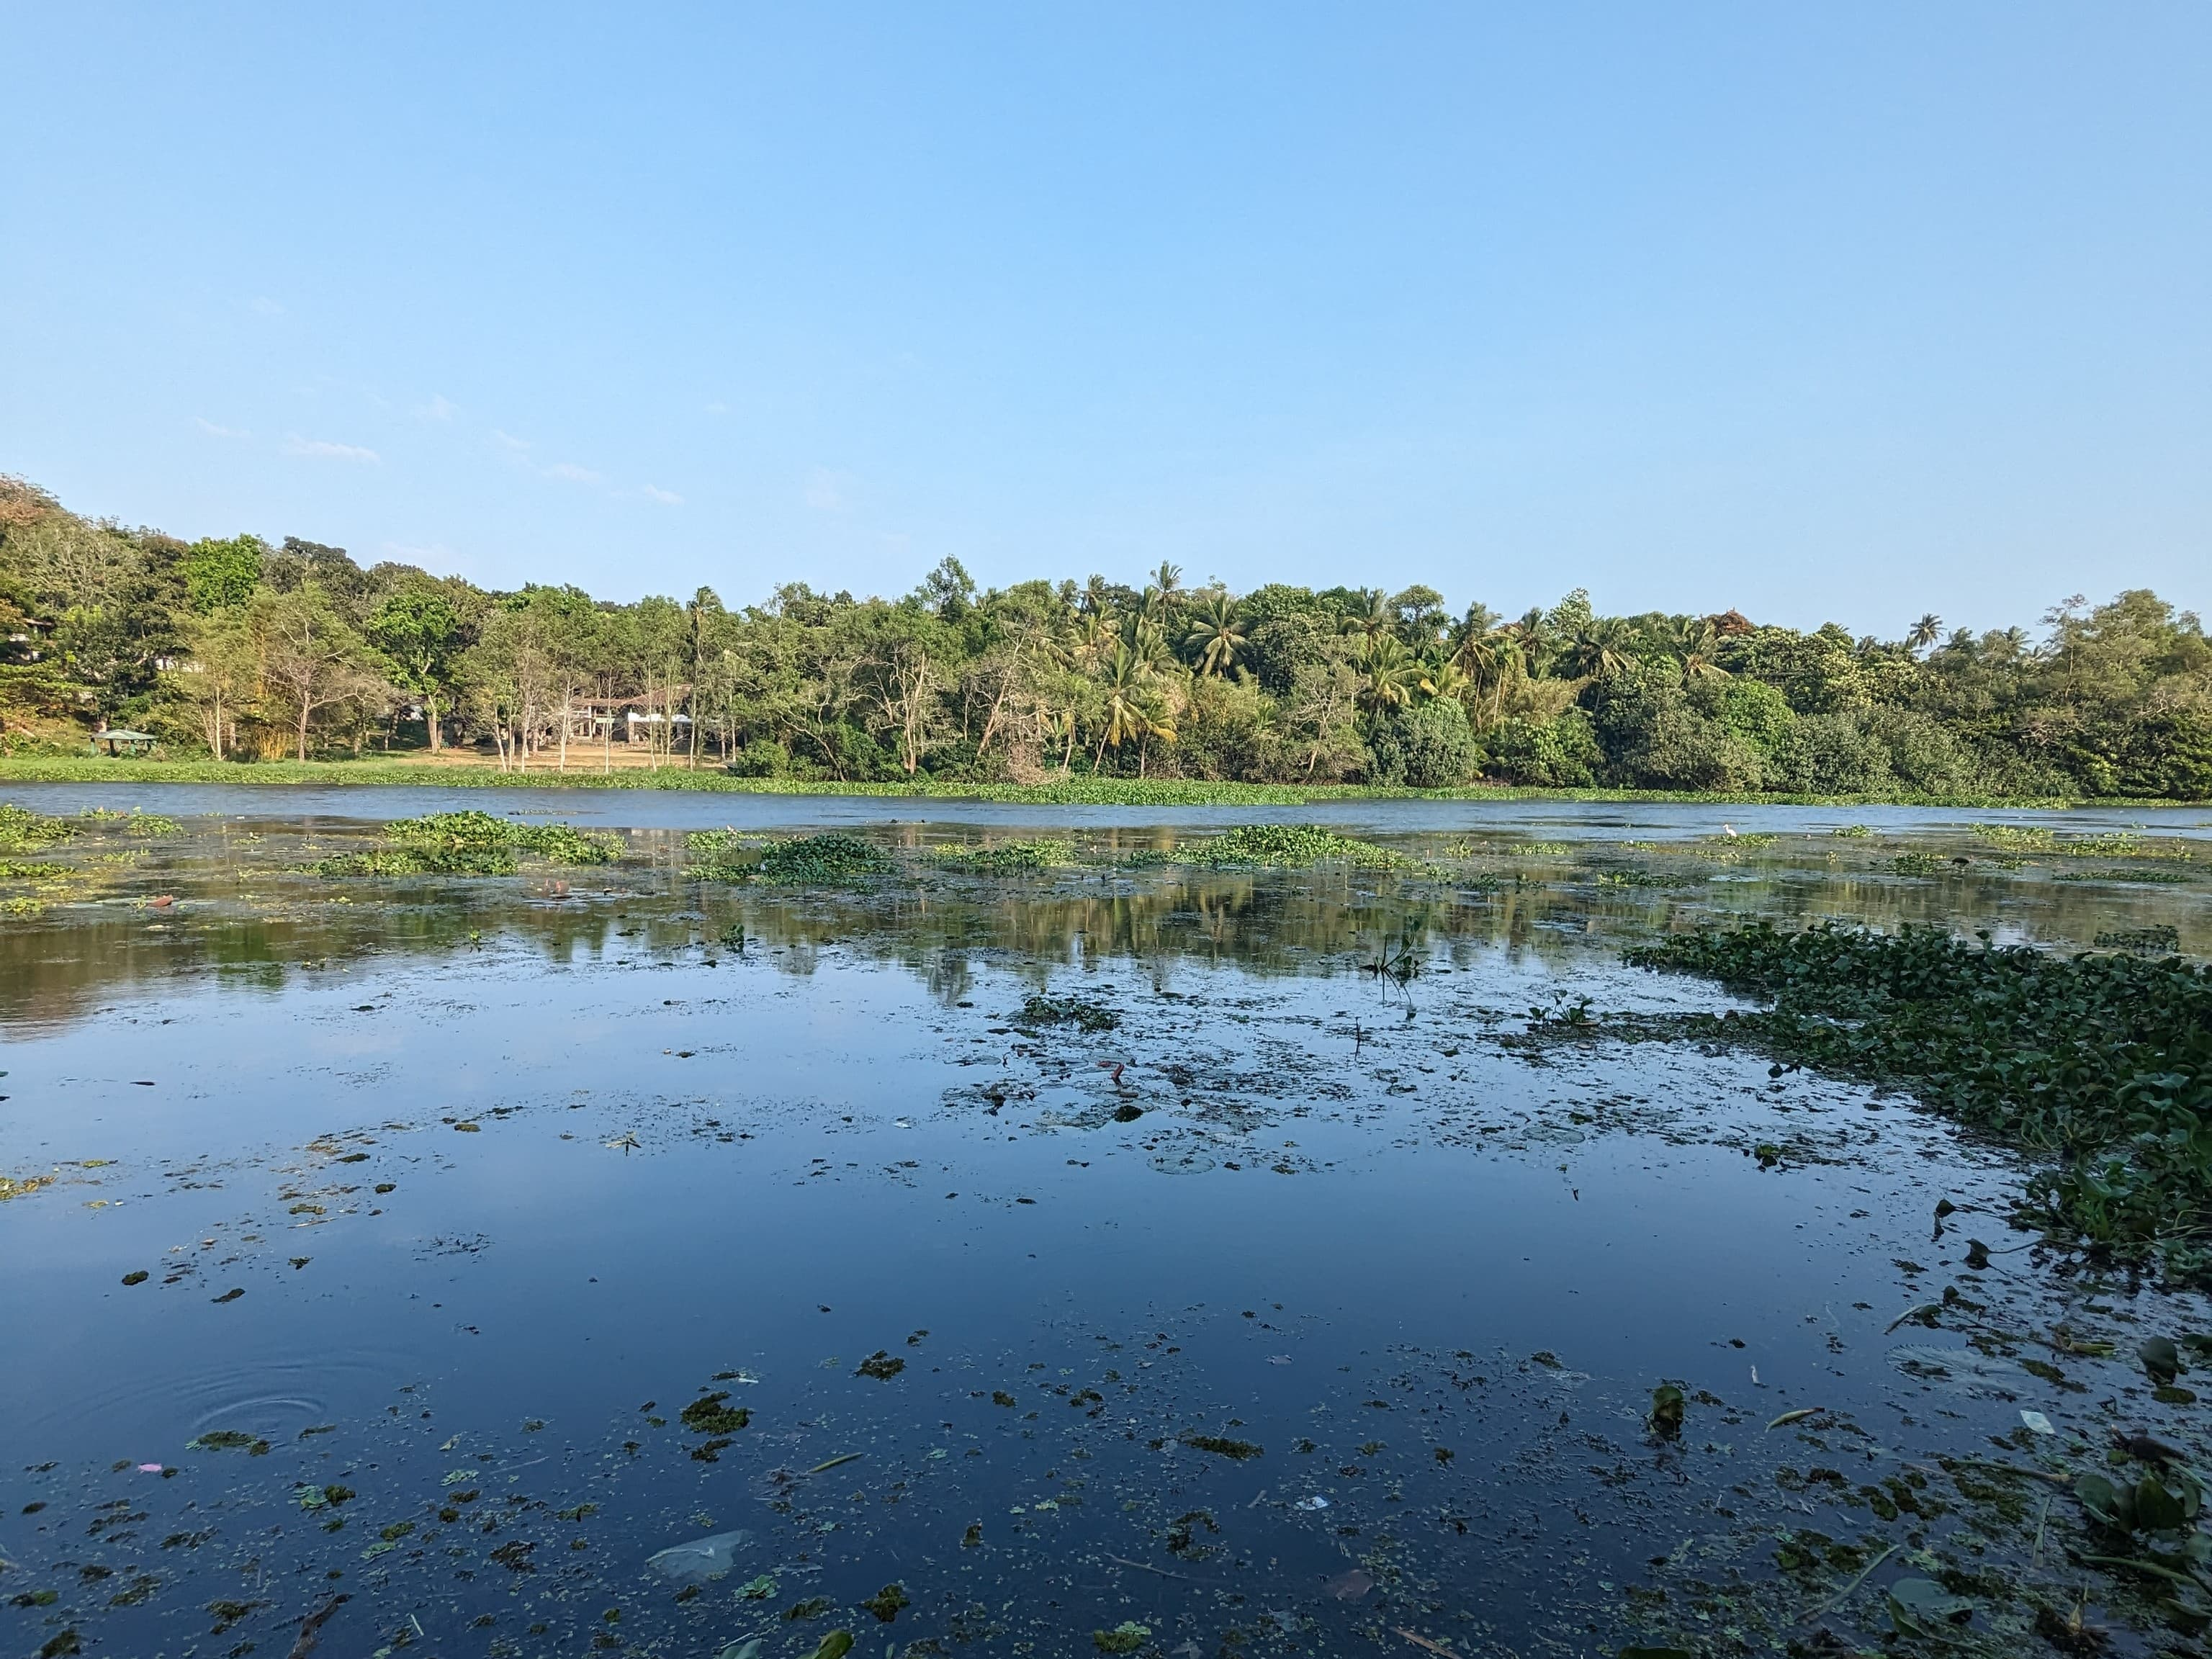
\includegraphics[width=\textwidth]{Figures/bolgoda.jpg}
        \caption{Bolgoda Lake view from the "Boat yard"}
        \label{fig:figure-02.1}
    \end{subfigure}
    \hspace{.5cm} % Adjust the space as needed
    \begin{subfigure}{0.45\textwidth}
        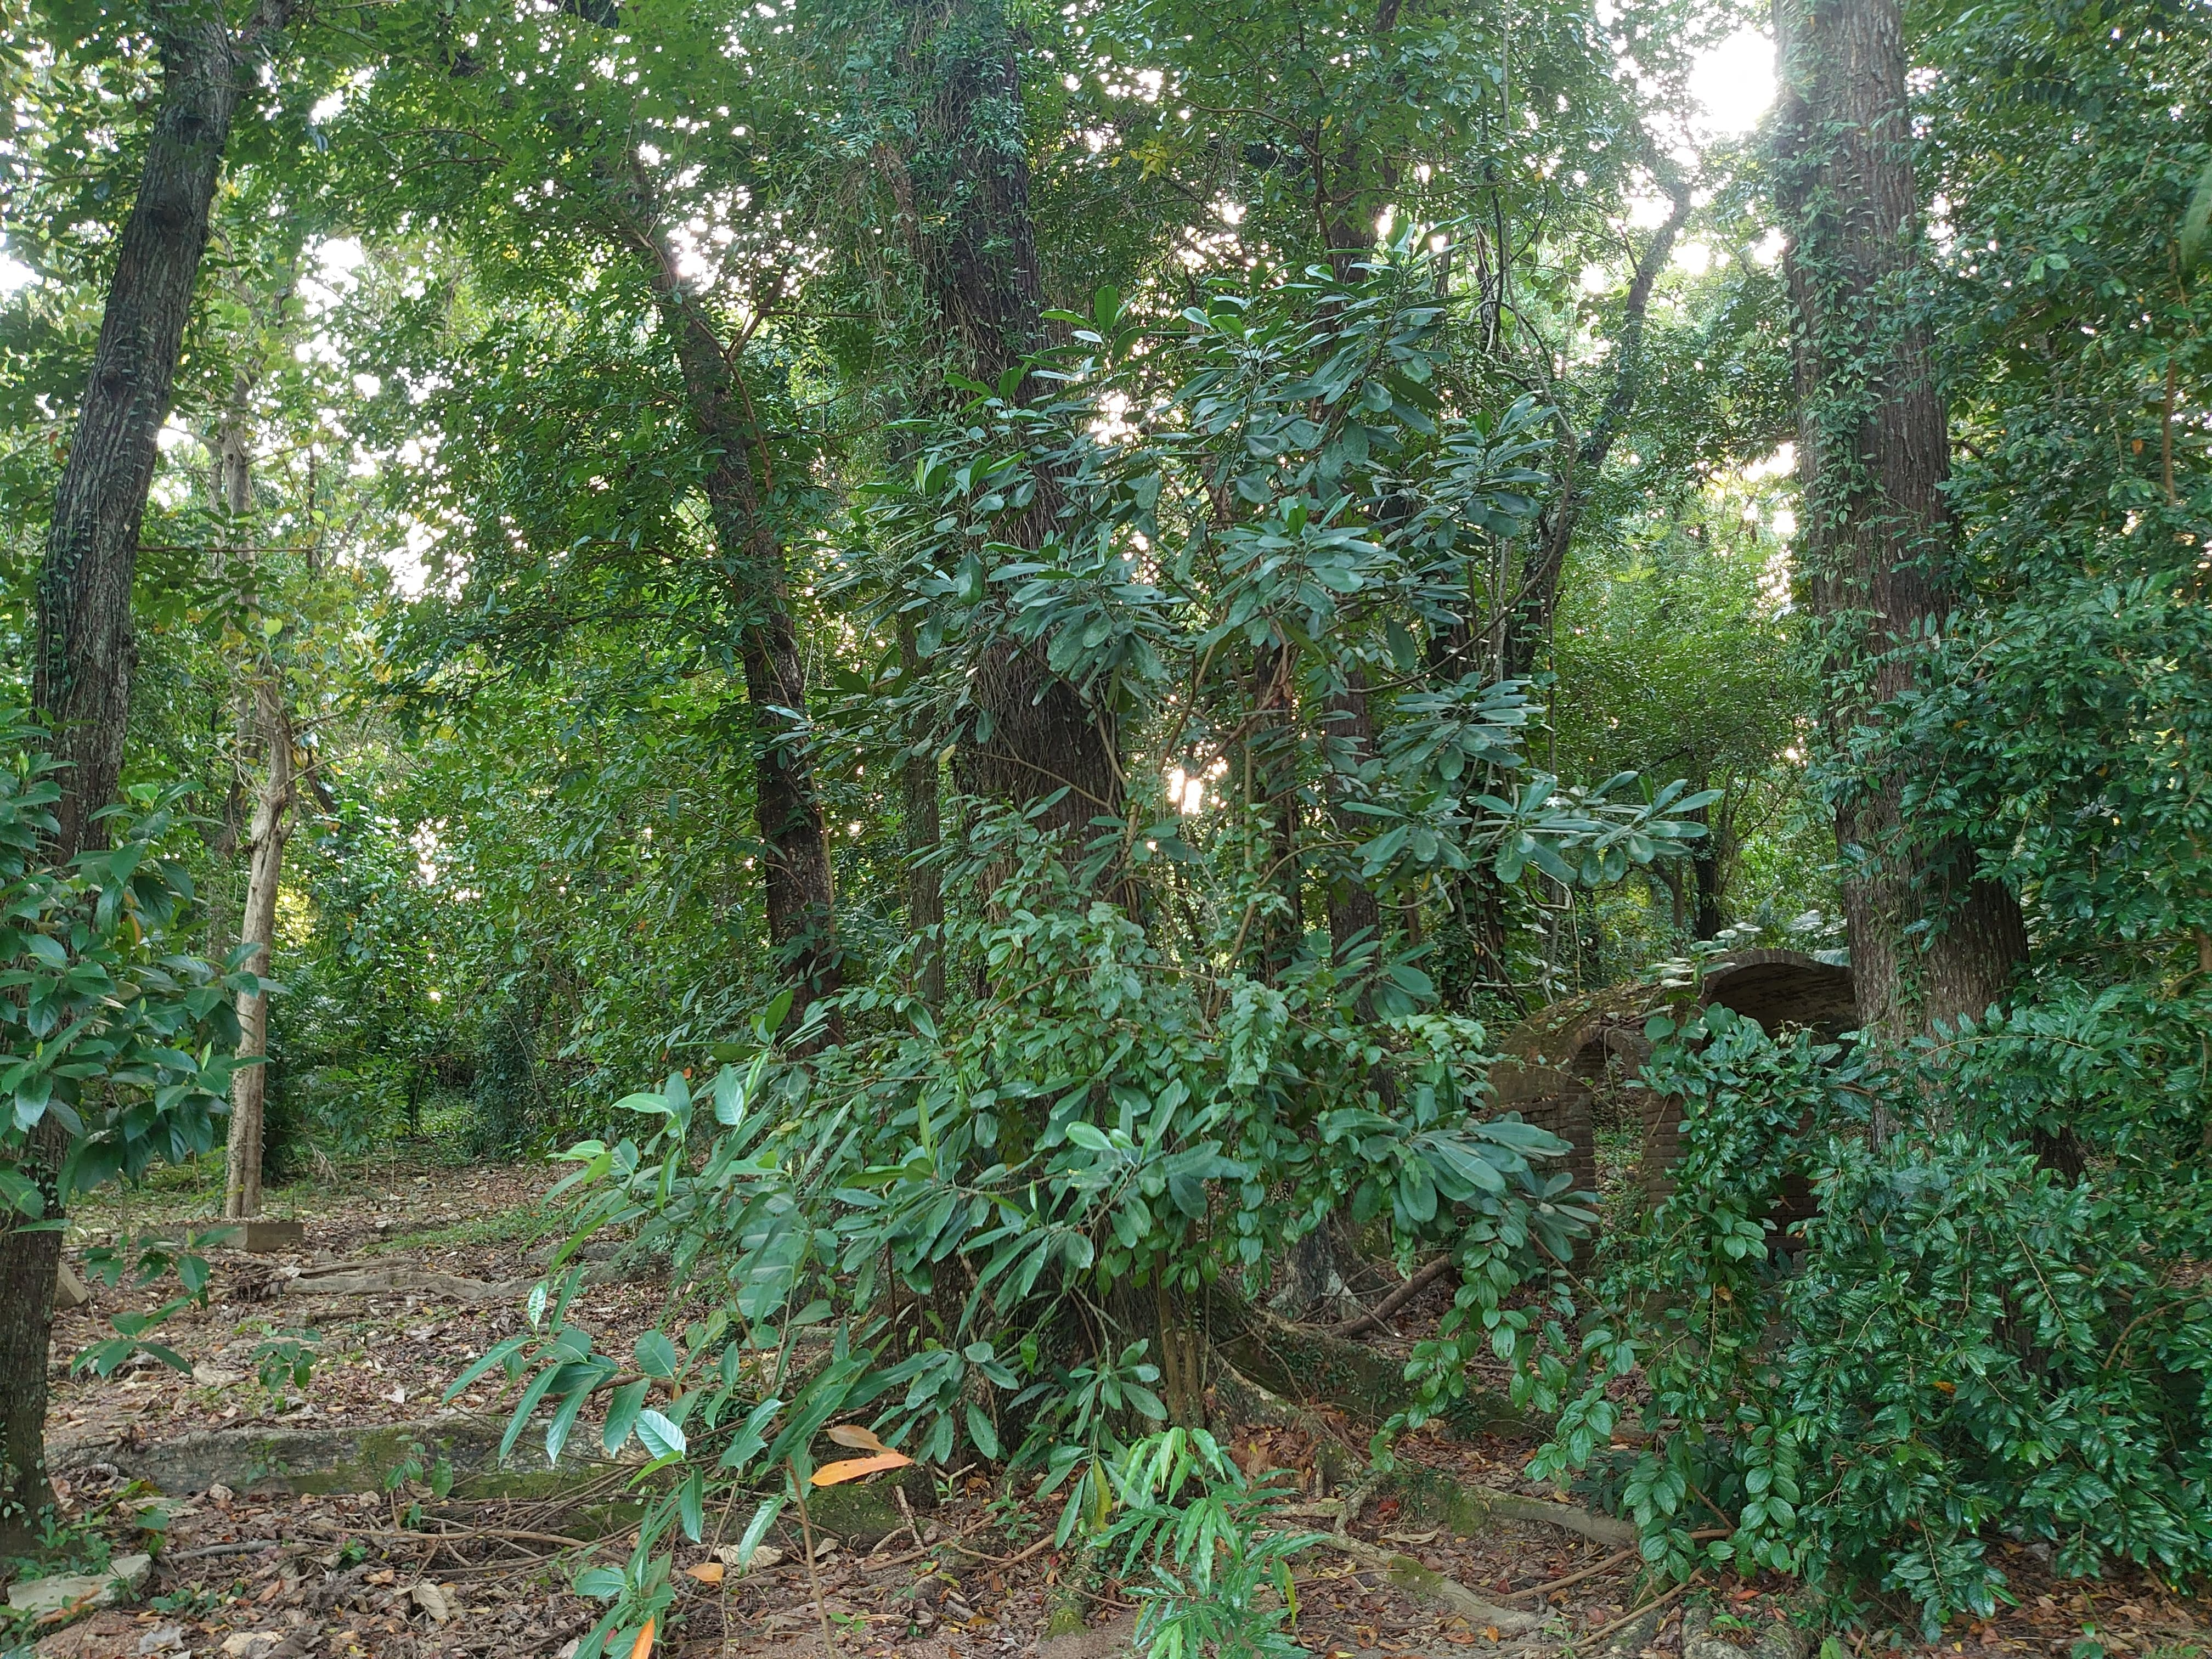
\includegraphics[width=\textwidth]{Figures/kajuKele.jpg}
        \caption{"Kaju Kele" forest patch}
        \label{fig:figure-02.2}
    \end{subfigure}
    \caption{Prominent natural Eco Systems in the University}
    \label{fig:figure-02}
\end{figure}

\subsection{Hotspots}
During the study two hotspots was identified inside the above eco systems which has been the locations where exceptionally high number of bird species was documented.
\begin{enumerate}
    \item  Boat Yard and the Open land stripe with a lineup of trees between Department of Civil Engineering and the Bolgoda lake.
    \item The open area located near the first security guard room inside "Kaju kele" when entered from the side where the boat yard is located.
\end{enumerate}